% Options for packages loaded elsewhere
\PassOptionsToPackage{unicode}{hyperref}
\PassOptionsToPackage{hyphens}{url}
%
\documentclass[
]{article}
\usepackage{amsmath,amssymb}
\usepackage{iftex}
\ifPDFTeX
  \usepackage[T1]{fontenc}
  \usepackage[utf8]{inputenc}
  \usepackage{textcomp} % provide euro and other symbols
\else % if luatex or xetex
  \usepackage{unicode-math} % this also loads fontspec
  \defaultfontfeatures{Scale=MatchLowercase}
  \defaultfontfeatures[\rmfamily]{Ligatures=TeX,Scale=1}
\fi
\usepackage{lmodern}
\ifPDFTeX\else
  % xetex/luatex font selection
\fi
% Use upquote if available, for straight quotes in verbatim environments
\IfFileExists{upquote.sty}{\usepackage{upquote}}{}
\IfFileExists{microtype.sty}{% use microtype if available
  \usepackage[]{microtype}
  \UseMicrotypeSet[protrusion]{basicmath} % disable protrusion for tt fonts
}{}
\makeatletter
\@ifundefined{KOMAClassName}{% if non-KOMA class
  \IfFileExists{parskip.sty}{%
    \usepackage{parskip}
  }{% else
    \setlength{\parindent}{0pt}
    \setlength{\parskip}{6pt plus 2pt minus 1pt}}
}{% if KOMA class
  \KOMAoptions{parskip=half}}
\makeatother
\usepackage{xcolor}
\usepackage[margin=1in]{geometry}
\usepackage{color}
\usepackage{fancyvrb}
\newcommand{\VerbBar}{|}
\newcommand{\VERB}{\Verb[commandchars=\\\{\}]}
\DefineVerbatimEnvironment{Highlighting}{Verbatim}{commandchars=\\\{\}}
% Add ',fontsize=\small' for more characters per line
\usepackage{framed}
\definecolor{shadecolor}{RGB}{248,248,248}
\newenvironment{Shaded}{\begin{snugshade}}{\end{snugshade}}
\newcommand{\AlertTok}[1]{\textcolor[rgb]{0.94,0.16,0.16}{#1}}
\newcommand{\AnnotationTok}[1]{\textcolor[rgb]{0.56,0.35,0.01}{\textbf{\textit{#1}}}}
\newcommand{\AttributeTok}[1]{\textcolor[rgb]{0.13,0.29,0.53}{#1}}
\newcommand{\BaseNTok}[1]{\textcolor[rgb]{0.00,0.00,0.81}{#1}}
\newcommand{\BuiltInTok}[1]{#1}
\newcommand{\CharTok}[1]{\textcolor[rgb]{0.31,0.60,0.02}{#1}}
\newcommand{\CommentTok}[1]{\textcolor[rgb]{0.56,0.35,0.01}{\textit{#1}}}
\newcommand{\CommentVarTok}[1]{\textcolor[rgb]{0.56,0.35,0.01}{\textbf{\textit{#1}}}}
\newcommand{\ConstantTok}[1]{\textcolor[rgb]{0.56,0.35,0.01}{#1}}
\newcommand{\ControlFlowTok}[1]{\textcolor[rgb]{0.13,0.29,0.53}{\textbf{#1}}}
\newcommand{\DataTypeTok}[1]{\textcolor[rgb]{0.13,0.29,0.53}{#1}}
\newcommand{\DecValTok}[1]{\textcolor[rgb]{0.00,0.00,0.81}{#1}}
\newcommand{\DocumentationTok}[1]{\textcolor[rgb]{0.56,0.35,0.01}{\textbf{\textit{#1}}}}
\newcommand{\ErrorTok}[1]{\textcolor[rgb]{0.64,0.00,0.00}{\textbf{#1}}}
\newcommand{\ExtensionTok}[1]{#1}
\newcommand{\FloatTok}[1]{\textcolor[rgb]{0.00,0.00,0.81}{#1}}
\newcommand{\FunctionTok}[1]{\textcolor[rgb]{0.13,0.29,0.53}{\textbf{#1}}}
\newcommand{\ImportTok}[1]{#1}
\newcommand{\InformationTok}[1]{\textcolor[rgb]{0.56,0.35,0.01}{\textbf{\textit{#1}}}}
\newcommand{\KeywordTok}[1]{\textcolor[rgb]{0.13,0.29,0.53}{\textbf{#1}}}
\newcommand{\NormalTok}[1]{#1}
\newcommand{\OperatorTok}[1]{\textcolor[rgb]{0.81,0.36,0.00}{\textbf{#1}}}
\newcommand{\OtherTok}[1]{\textcolor[rgb]{0.56,0.35,0.01}{#1}}
\newcommand{\PreprocessorTok}[1]{\textcolor[rgb]{0.56,0.35,0.01}{\textit{#1}}}
\newcommand{\RegionMarkerTok}[1]{#1}
\newcommand{\SpecialCharTok}[1]{\textcolor[rgb]{0.81,0.36,0.00}{\textbf{#1}}}
\newcommand{\SpecialStringTok}[1]{\textcolor[rgb]{0.31,0.60,0.02}{#1}}
\newcommand{\StringTok}[1]{\textcolor[rgb]{0.31,0.60,0.02}{#1}}
\newcommand{\VariableTok}[1]{\textcolor[rgb]{0.00,0.00,0.00}{#1}}
\newcommand{\VerbatimStringTok}[1]{\textcolor[rgb]{0.31,0.60,0.02}{#1}}
\newcommand{\WarningTok}[1]{\textcolor[rgb]{0.56,0.35,0.01}{\textbf{\textit{#1}}}}
\usepackage{graphicx}
\makeatletter
\def\maxwidth{\ifdim\Gin@nat@width>\linewidth\linewidth\else\Gin@nat@width\fi}
\def\maxheight{\ifdim\Gin@nat@height>\textheight\textheight\else\Gin@nat@height\fi}
\makeatother
% Scale images if necessary, so that they will not overflow the page
% margins by default, and it is still possible to overwrite the defaults
% using explicit options in \includegraphics[width, height, ...]{}
\setkeys{Gin}{width=\maxwidth,height=\maxheight,keepaspectratio}
% Set default figure placement to htbp
\makeatletter
\def\fps@figure{htbp}
\makeatother
\setlength{\emergencystretch}{3em} % prevent overfull lines
\providecommand{\tightlist}{%
  \setlength{\itemsep}{0pt}\setlength{\parskip}{0pt}}
\setcounter{secnumdepth}{-\maxdimen} % remove section numbering
\ifLuaTeX
  \usepackage{selnolig}  % disable illegal ligatures
\fi
\IfFileExists{bookmark.sty}{\usepackage{bookmark}}{\usepackage{hyperref}}
\IfFileExists{xurl.sty}{\usepackage{xurl}}{} % add URL line breaks if available
\urlstyle{same}
\hypersetup{
  pdftitle={Reproducible Research: Peer Assessment 1},
  hidelinks,
  pdfcreator={LaTeX via pandoc}}

\title{Reproducible Research: Peer Assessment 1}
\author{}
\date{\vspace{-2.5em}}

\begin{document}
\maketitle

\hypertarget{environment}{%
\subsection{Environment}\label{environment}}

\begin{Shaded}
\begin{Highlighting}[]
\FunctionTok{library}\NormalTok{(magrittr)}
\FunctionTok{library}\NormalTok{(dplyr)}
\FunctionTok{library}\NormalTok{(ggplot2)}
\FunctionTok{library}\NormalTok{(scales)}
\FunctionTok{library}\NormalTok{(ggplot2)}
\FunctionTok{library}\NormalTok{(knitr)}
\end{Highlighting}
\end{Shaded}

\hypertarget{loading-and-preprocessing-the-data}{%
\subsection{Loading and preprocessing the
data}\label{loading-and-preprocessing-the-data}}

\begin{Shaded}
\begin{Highlighting}[]
\CommentTok{\# Load the activity data}
\NormalTok{data }\OtherTok{\textless{}{-}} \FunctionTok{read.csv}\NormalTok{(}\StringTok{"activity.csv"}\NormalTok{)}

\CommentTok{\# Preprocess the data}
\NormalTok{data }\SpecialCharTok{\%\textless{}\textgreater{}\%}
  \FunctionTok{mutate}\NormalTok{(}\AttributeTok{date=}\FunctionTok{as.Date}\NormalTok{(}\FunctionTok{as.character}\NormalTok{(date, }\AttributeTok{format=}\StringTok{"\%Y\%m\%d"}\NormalTok{)))}
\end{Highlighting}
\end{Shaded}

\hypertarget{what-is-mean-total-number-of-steps-taken-per-day}{%
\subsection{What is mean total number of steps taken per
day?}\label{what-is-mean-total-number-of-steps-taken-per-day}}

\begin{Shaded}
\begin{Highlighting}[]
\CommentTok{\# Group steps by day}
\NormalTok{data\_grouped\_day }\OtherTok{\textless{}{-}}\NormalTok{ data }\SpecialCharTok{\%\textgreater{}\%} 
  \FunctionTok{group\_by}\NormalTok{(date) }\SpecialCharTok{\%\textgreater{}\%} 
  \FunctionTok{summarize}\NormalTok{(}
    \AttributeTok{steps=}\FunctionTok{sum}\NormalTok{(steps, }\AttributeTok{na.rm=}\ConstantTok{TRUE}\NormalTok{)}
\NormalTok{  )}

\CommentTok{\# Plot histogram}
\FunctionTok{png}\NormalTok{(}\StringTok{"figures/plot1.png"}\NormalTok{)}
\FunctionTok{hist}\NormalTok{(data\_grouped\_day}\SpecialCharTok{$}\NormalTok{steps, }\AttributeTok{breaks=}\DecValTok{30}\NormalTok{, }\AttributeTok{xlab=}\StringTok{"date"}\NormalTok{, }\AttributeTok{ylab=}\StringTok{"steps"}\NormalTok{, }\AttributeTok{main=}\StringTok{"Total number of steps taken each day"}\NormalTok{)}
\FunctionTok{dev.off}\NormalTok{()}
\end{Highlighting}
\end{Shaded}

\begin{verbatim}
## pdf 
##   2
\end{verbatim}

\begin{Shaded}
\begin{Highlighting}[]
\FunctionTok{hist}\NormalTok{(data\_grouped\_day}\SpecialCharTok{$}\NormalTok{steps, }\AttributeTok{breaks=}\DecValTok{30}\NormalTok{, }\AttributeTok{xlab=}\StringTok{"date"}\NormalTok{, }\AttributeTok{ylab=}\StringTok{"steps"}\NormalTok{, }\AttributeTok{main=}\StringTok{"Total number of steps taken each day"}\NormalTok{)}
\end{Highlighting}
\end{Shaded}

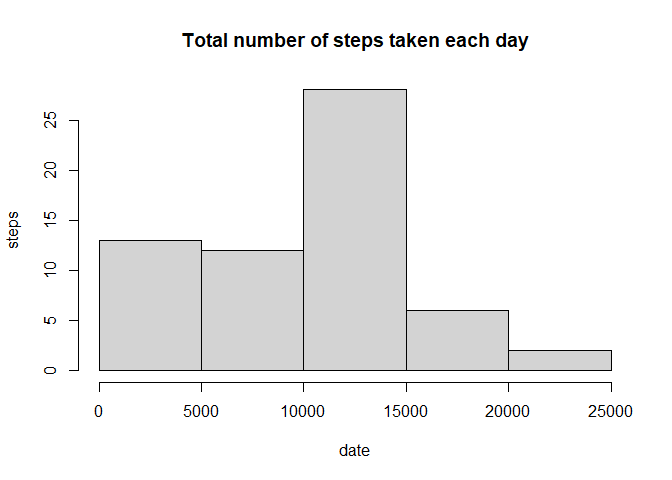
\includegraphics{PA1_template_files/figure-latex/unnamed-chunk-3-1.pdf}

\begin{Shaded}
\begin{Highlighting}[]
\CommentTok{\# Print mean and median steps per day}
\NormalTok{mean\_before\_imput }\OtherTok{\textless{}{-}} \FunctionTok{round}\NormalTok{(}\FunctionTok{mean}\NormalTok{(data\_grouped\_day}\SpecialCharTok{$}\NormalTok{steps), }\DecValTok{0}\NormalTok{)}
\NormalTok{median\_before\_imput }\OtherTok{\textless{}{-}} \FunctionTok{round}\NormalTok{(}\FunctionTok{median}\NormalTok{(data\_grouped\_day}\SpecialCharTok{$}\NormalTok{steps), }\DecValTok{0}\NormalTok{)}
\FunctionTok{cat}\NormalTok{(}\FunctionTok{sprintf}\NormalTok{(}\StringTok{\textquotesingle{}The mean steps taken per day is \%d}\SpecialCharTok{\textbackslash{}n}\StringTok{\textquotesingle{}}\NormalTok{, mean\_before\_imput))}
\end{Highlighting}
\end{Shaded}

\begin{verbatim}
## The mean steps taken per day is 9354
\end{verbatim}

\begin{Shaded}
\begin{Highlighting}[]
\FunctionTok{cat}\NormalTok{(}\FunctionTok{sprintf}\NormalTok{(}\StringTok{\textquotesingle{}The mean steps taken per day is \%d\textquotesingle{}}\NormalTok{, median\_before\_imput))}
\end{Highlighting}
\end{Shaded}

\begin{verbatim}
## The mean steps taken per day is 10395
\end{verbatim}

\hypertarget{what-is-the-average-daily-activity-pattern}{%
\subsection{What is the average daily activity
pattern?}\label{what-is-the-average-daily-activity-pattern}}

\begin{Shaded}
\begin{Highlighting}[]
\CommentTok{\# Group steps by day}
\NormalTok{data\_grouped\_interval }\OtherTok{\textless{}{-}}\NormalTok{ data }\SpecialCharTok{\%\textgreater{}\%} 
  \FunctionTok{group\_by}\NormalTok{(interval) }\SpecialCharTok{\%\textgreater{}\%} 
  \FunctionTok{summarize}\NormalTok{(}
    \AttributeTok{steps=}\FunctionTok{mean}\NormalTok{(steps, }\AttributeTok{na.rm=}\ConstantTok{TRUE}\NormalTok{)}
\NormalTok{  )}

\CommentTok{\# Plot histogram}
\FunctionTok{png}\NormalTok{(}\StringTok{"figures/plot2.png"}\NormalTok{)}
\FunctionTok{with}\NormalTok{(data\_grouped\_interval, }\FunctionTok{plot}\NormalTok{(}\AttributeTok{x=}\NormalTok{interval, }\AttributeTok{y=}\NormalTok{steps, }\AttributeTok{type=}\StringTok{"l"}\NormalTok{, }\AttributeTok{xlab=}\StringTok{"interval"}\NormalTok{, }\AttributeTok{ylab=}\StringTok{"steps"}\NormalTok{, }\AttributeTok{main=}\StringTok{"Time series plot of average number of steps taken by day intervals"}\NormalTok{))}
\FunctionTok{dev.off}\NormalTok{()}
\end{Highlighting}
\end{Shaded}

\begin{verbatim}
## pdf 
##   2
\end{verbatim}

\begin{Shaded}
\begin{Highlighting}[]
\FunctionTok{with}\NormalTok{(data\_grouped\_interval, }\FunctionTok{plot}\NormalTok{(}\AttributeTok{x=}\NormalTok{interval, }\AttributeTok{y=}\NormalTok{steps, }\AttributeTok{type=}\StringTok{"l"}\NormalTok{, }\AttributeTok{xlab=}\StringTok{"interval"}\NormalTok{, }\AttributeTok{ylab=}\StringTok{"steps"}\NormalTok{, }\AttributeTok{main=}\StringTok{"Time series plot of average number of steps taken by day intervals"}\NormalTok{))}
\end{Highlighting}
\end{Shaded}

\includegraphics{PA1_template_files/figure-latex/unnamed-chunk-4-1.pdf}

\begin{Shaded}
\begin{Highlighting}[]
\CommentTok{\# Find interval with max steps}
\NormalTok{max\_steps }\OtherTok{\textless{}{-}} \FunctionTok{subset}\NormalTok{(data\_grouped\_interval, steps}\SpecialCharTok{==}\FunctionTok{max}\NormalTok{(steps))}

\CommentTok{\# Print mean and median steps per day}
\FunctionTok{cat}\NormalTok{(}\FunctionTok{sprintf}\NormalTok{(}\StringTok{\textquotesingle{}The 5{-}minute interval, on average across all the days in the dataset, that contains the maximum number of steps is \%d\textquotesingle{}}\NormalTok{, max\_steps}\SpecialCharTok{$}\NormalTok{interval))}
\end{Highlighting}
\end{Shaded}

\begin{verbatim}
## The 5-minute interval, on average across all the days in the dataset, that contains the maximum number of steps is 835
\end{verbatim}

\hypertarget{imputing-missing-values}{%
\subsection{Imputing missing values}\label{imputing-missing-values}}

\begin{Shaded}
\begin{Highlighting}[]
\CommentTok{\# Print nº of NA}
\FunctionTok{cat}\NormalTok{(}\FunctionTok{sprintf}\NormalTok{(}\StringTok{\textquotesingle{}The total number of missing values in the dataset is \%d}\SpecialCharTok{\textbackslash{}n}\StringTok{\textquotesingle{}}\NormalTok{, }\FunctionTok{sum}\NormalTok{(}\FunctionTok{is.na}\NormalTok{(data}\SpecialCharTok{$}\NormalTok{steps))))}
\end{Highlighting}
\end{Shaded}

\begin{verbatim}
## The total number of missing values in the dataset is 2304
\end{verbatim}

\begin{Shaded}
\begin{Highlighting}[]
\CommentTok{\# Calculate mean per 5{-}minute interval and impute steps by interval mean}
\NormalTok{data\_mean\_interval }\OtherTok{\textless{}{-}}\NormalTok{ data }\SpecialCharTok{\%\textgreater{}\%}
  \FunctionTok{group\_by}\NormalTok{(interval) }\SpecialCharTok{\%\textgreater{}\%}
  \FunctionTok{mutate}\NormalTok{(}\AttributeTok{mean\_interval =} \FunctionTok{round}\NormalTok{(}\FunctionTok{mean}\NormalTok{(steps, }\AttributeTok{na.rm =} \ConstantTok{TRUE}\NormalTok{),}\DecValTok{0}\NormalTok{)) }\SpecialCharTok{\%\textgreater{}\%} 
  \FunctionTok{ungroup}\NormalTok{() }\SpecialCharTok{\%\textgreater{}\%} 
  \FunctionTok{mutate}\NormalTok{(}\AttributeTok{steps=}\FunctionTok{ifelse}\NormalTok{(}\FunctionTok{is.na}\NormalTok{(steps), mean\_interval, steps))}

\CommentTok{\# Group by day}
\NormalTok{data\_grouped\_day\_imputed }\OtherTok{\textless{}{-}}\NormalTok{ data\_mean\_interval }\SpecialCharTok{\%\textgreater{}\%} 
  \FunctionTok{group\_by}\NormalTok{(date) }\SpecialCharTok{\%\textgreater{}\%} 
  \FunctionTok{summarize}\NormalTok{(}
    \AttributeTok{steps=}\FunctionTok{sum}\NormalTok{(steps, }\AttributeTok{na.rm=}\ConstantTok{TRUE}\NormalTok{)}
\NormalTok{  )}

\CommentTok{\# Plot histogram}
\FunctionTok{png}\NormalTok{(}\StringTok{"figures/plot3.png"}\NormalTok{)}
\FunctionTok{hist}\NormalTok{(data\_grouped\_day\_imputed}\SpecialCharTok{$}\NormalTok{steps, }\AttributeTok{breaks=}\DecValTok{30}\NormalTok{, }\AttributeTok{xlab=}\StringTok{"date"}\NormalTok{, }\AttributeTok{ylab=}\StringTok{"steps"}\NormalTok{, }\AttributeTok{main=}\StringTok{"Total number of steps taken each day"}\NormalTok{)}
\FunctionTok{dev.off}\NormalTok{()}
\end{Highlighting}
\end{Shaded}

\begin{verbatim}
## pdf 
##   2
\end{verbatim}

\begin{Shaded}
\begin{Highlighting}[]
\FunctionTok{hist}\NormalTok{(data\_grouped\_day\_imputed}\SpecialCharTok{$}\NormalTok{steps, }\AttributeTok{breaks=}\DecValTok{30}\NormalTok{, }\AttributeTok{xlab=}\StringTok{"date"}\NormalTok{, }\AttributeTok{ylab=}\StringTok{"steps"}\NormalTok{, }\AttributeTok{main=}\StringTok{"Total number of steps taken each day"}\NormalTok{)}
\end{Highlighting}
\end{Shaded}

\includegraphics{PA1_template_files/figure-latex/unnamed-chunk-5-1.pdf}

\begin{Shaded}
\begin{Highlighting}[]
\CommentTok{\# Print mean and median steps per day after imputing}
\NormalTok{mean\_after\_imput }\OtherTok{\textless{}{-}} \FunctionTok{round}\NormalTok{(}\FunctionTok{mean}\NormalTok{(data\_grouped\_day\_imputed}\SpecialCharTok{$}\NormalTok{steps), }\DecValTok{0}\NormalTok{)}
\NormalTok{median\_after\_imput }\OtherTok{\textless{}{-}} \FunctionTok{round}\NormalTok{(}\FunctionTok{median}\NormalTok{(data\_grouped\_day\_imputed}\SpecialCharTok{$}\NormalTok{steps), }\DecValTok{0}\NormalTok{)}
\FunctionTok{cat}\NormalTok{(}\FunctionTok{sprintf}\NormalTok{(}\StringTok{\textquotesingle{}The mean steps taken per day is \%d}\SpecialCharTok{\textbackslash{}n}\StringTok{\textquotesingle{}}\NormalTok{, mean\_after\_imput))}
\end{Highlighting}
\end{Shaded}

\begin{verbatim}
## The mean steps taken per day is 10766
\end{verbatim}

\begin{Shaded}
\begin{Highlighting}[]
\FunctionTok{cat}\NormalTok{(}\FunctionTok{sprintf}\NormalTok{(}\StringTok{\textquotesingle{}The mean steps taken per day is \%d}\SpecialCharTok{\textbackslash{}n}\StringTok{\textquotesingle{}}\NormalTok{, median\_after\_imput))}
\end{Highlighting}
\end{Shaded}

\begin{verbatim}
## The mean steps taken per day is 10762
\end{verbatim}

\begin{Shaded}
\begin{Highlighting}[]
\CommentTok{\# Differences between mean and median before and after imputing}
\ControlFlowTok{if}\NormalTok{ (mean\_after\_imput }\SpecialCharTok{\textgreater{}}\NormalTok{ mean\_before\_imput) \{}
  \FunctionTok{print}\NormalTok{(}\StringTok{"Mean after imputation is higher than mean before imputation"}\NormalTok{)}
\NormalTok{\} }\ControlFlowTok{else} \ControlFlowTok{if}\NormalTok{ (mean\_after\_imput }\SpecialCharTok{\textless{}}\NormalTok{ mean\_before\_imput) \{}
  \FunctionTok{print}\NormalTok{(}\StringTok{"Mean after imputation is lower than mean before imputation"}\NormalTok{)}
\NormalTok{\} }\ControlFlowTok{else}\NormalTok{ \{}
  \FunctionTok{print}\NormalTok{(}\StringTok{"Mean did not change after imputation"}\NormalTok{)}
\NormalTok{\}}
\end{Highlighting}
\end{Shaded}

\begin{verbatim}
## [1] "Mean after imputation is higher than mean before imputation"
\end{verbatim}

\begin{Shaded}
\begin{Highlighting}[]
\ControlFlowTok{if}\NormalTok{ (median\_after\_imput }\SpecialCharTok{\textgreater{}}\NormalTok{ median\_before\_imput) \{}
  \FunctionTok{print}\NormalTok{(}\StringTok{"Median after imputation is higher than median before imputation"}\NormalTok{)}
\NormalTok{\} }\ControlFlowTok{else} \ControlFlowTok{if}\NormalTok{ (median\_after\_imput }\SpecialCharTok{\textless{}}\NormalTok{ median\_before\_imput) \{}
  \FunctionTok{print}\NormalTok{(}\StringTok{"Median after imputation is lower than median before imputation"}\NormalTok{)}
\NormalTok{\} }\ControlFlowTok{else}\NormalTok{ \{}
  \FunctionTok{print}\NormalTok{(}\StringTok{"Median did not change after imputation"}\NormalTok{)}
\NormalTok{\}}
\end{Highlighting}
\end{Shaded}

\begin{verbatim}
## [1] "Median after imputation is higher than median before imputation"
\end{verbatim}

\hypertarget{are-there-differences-in-activity-patterns-between-weekdays-and-weekends}{%
\subsection{Are there differences in activity patterns between weekdays
and
weekends?}\label{are-there-differences-in-activity-patterns-between-weekdays-and-weekends}}

\begin{Shaded}
\begin{Highlighting}[]
\CommentTok{\# Create dataframe with type of day}
\NormalTok{data\_grouped\_day\_imputed\_weekday }\OtherTok{\textless{}{-}}\NormalTok{ data\_mean\_interval }\SpecialCharTok{\%\textgreater{}\%} 
  \FunctionTok{mutate}\NormalTok{(}\AttributeTok{day\_type =} \FunctionTok{ifelse}\NormalTok{(}\FunctionTok{weekdays}\NormalTok{(date) }\SpecialCharTok{\%in\%} \FunctionTok{c}\NormalTok{(}\StringTok{"lunes"}\NormalTok{, }\StringTok{"martes"}\NormalTok{, }\StringTok{"miércoles"}\NormalTok{, }\StringTok{"jueves"}\NormalTok{, }\StringTok{"viernes"}\NormalTok{), }\StringTok{"weekday"}\NormalTok{, }\StringTok{"weekend"}\NormalTok{)) }\SpecialCharTok{\%\textgreater{}\%}
  \FunctionTok{mutate}\NormalTok{(}\AttributeTok{day\_type =} \FunctionTok{as.factor}\NormalTok{(day\_type)) }\SpecialCharTok{\%\textgreater{}\%} 
  \FunctionTok{select}\NormalTok{(}\SpecialCharTok{{-}}\NormalTok{mean\_interval) }\SpecialCharTok{\%\textgreater{}\%}
  \FunctionTok{group\_by}\NormalTok{(interval, day\_type) }\SpecialCharTok{\%\textgreater{}\%} 
  \FunctionTok{summarize}\NormalTok{(}
    \AttributeTok{steps=}\FunctionTok{mean}\NormalTok{(steps, }\AttributeTok{na.rm=}\ConstantTok{TRUE}\NormalTok{)}
\NormalTok{  )}
\end{Highlighting}
\end{Shaded}

\begin{verbatim}
## `summarise()` has grouped output by 'interval'. You can override using the `.groups` argument.
\end{verbatim}

\begin{Shaded}
\begin{Highlighting}[]
\CommentTok{\# Plot histogram}
\FunctionTok{ggplot}\NormalTok{(data\_grouped\_day\_imputed\_weekday, }\FunctionTok{aes}\NormalTok{(}\AttributeTok{x =}\NormalTok{ interval, }\AttributeTok{y =}\NormalTok{ steps, }\AttributeTok{col =}\NormalTok{ day\_type)) }\SpecialCharTok{+}
  \FunctionTok{geom\_line}\NormalTok{() }\SpecialCharTok{+}
  \FunctionTok{facet\_grid}\NormalTok{(. }\SpecialCharTok{\textasciitilde{}}\NormalTok{ day\_type) }\SpecialCharTok{+}
  \FunctionTok{labs}\NormalTok{(}\AttributeTok{x =} \StringTok{"Interval"}\NormalTok{, }\AttributeTok{y =} \StringTok{"Steps"}\NormalTok{, }\AttributeTok{title =} \StringTok{"Time series plot of average number of steps taken by day intervals,}\SpecialCharTok{\textbackslash{}n}\StringTok{classified into weekdays and weekend"}\NormalTok{) }\SpecialCharTok{+}
  \FunctionTok{scale\_color\_manual}\NormalTok{(}\AttributeTok{values =} \FunctionTok{c}\NormalTok{(}\StringTok{"blue"}\NormalTok{, }\StringTok{"red"}\NormalTok{)) }\SpecialCharTok{+}
  \FunctionTok{theme\_minimal}\NormalTok{()}
\end{Highlighting}
\end{Shaded}

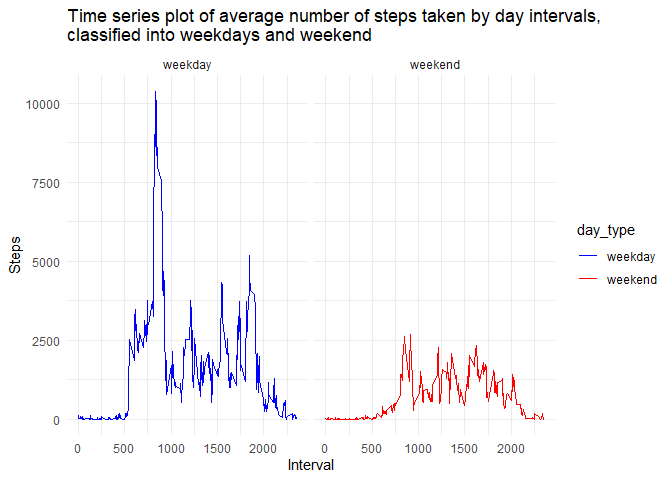
\includegraphics{PA1_template_files/figure-latex/unnamed-chunk-6-1.pdf}

\begin{Shaded}
\begin{Highlighting}[]
\FunctionTok{ggsave}\NormalTok{(}\StringTok{"figures/plot4.png"}\NormalTok{, }\AttributeTok{plot =} \FunctionTok{last\_plot}\NormalTok{(), }\AttributeTok{device =} \StringTok{"png"}\NormalTok{, }\AttributeTok{dpi =} \DecValTok{300}\NormalTok{)}
\end{Highlighting}
\end{Shaded}

\begin{verbatim}
## Saving 6.5 x 4.5 in image
\end{verbatim}

\end{document}
